% Discuss the PUF ROK and how it is relevant

\chapter{Read Once Keys}
\label{chapter:rok}

\section{Overview}
The term read-once keys (ROKs) describes the abstract notion that a cryptographic key can be read and used for encryption
and decryption only once. While it seems intuitive that a trusted piece of software could be designed that deletes a key right after
using it, such a scheme na\"{i}vely depends on the proper execution of the program. This approach could be easily
circumvented by running the code within a debugging environment that halts execution of the code before the deletion occurs.
That is, the notion of a ROK entails a stronger protection method wherein the process of reading the key 
results in its immediate destruction.

ROKs could be applied in a number of interesting scenarios. One application could be to create one-time programs~\cite{otp},
which could be beneficial for protecting the intellectual property of a piece of software. A potential client
could download a fully functional one-time program for evaluation before committing to a purchase.  A similar application
would be self-destructing email.  In that case, the sender could encrypt a message with a ROK; the message would then
be destroyed immediately after the recipient reads the message.  More generally, there is considerable interest in self-destructing
data, both commercially~\cite{ironkey} and academically~\cite{vanish}.  In addition, the use of trusted hardware tokens have been
proposed for applications including program obfuscation~\cite{obfusc}, monotonic counters~\cite{monotonictpm}, oblivious
transfer~\cite{ottamper}, and generalized secure computation~\cite{tamperhw}.  ROKs can provide the required functionality
for these applications.

Another interesting application of PUF ROKs is to defend against physical attacks on cryptographic protocols.  For example,
consider fault injection attacks on RSA~\cite{rsapub,pertrsa,insecrsa,rsaltr,fault}.  In these attacks, the algorithm is repeatedly executed
with the same key, using a controlled fault injection technique that will yield detectable differences in the output.  After enough such
iterations, the attacker is able to recover the key in full.  Similarly, ``freezing'' is another class of physical attack
that can extract a key if it was \emph{ever} stored in an accessible part of memory~\cite{freezing}.  PUF ROKs offer a unique defense against
all of these attacks because repeated execution with the same key cannot occur, and the key is \emph{never} actually present
in addressable physical memory.

The ability to generate ROKs in a controlled manner could also lead to an extension where keys can be generated and used
a multiple, but limited, number of times. For example, consider the use of ROKs to encrypt a public key {\it pk}. If an
identical ROK can be generated twice, the owner of {\it pk} could first use the key to create $e_{ROK}(pk)$ (indicating the
encryption of {\it pk} under with the ROK). Later, an authorized party could create the ROK a second time to decrypt the
key. Such a scheme could be used to delegate the authority to cryptographically sign documents.

In a sense, a ROK is an example of a program obfuscator.  An obfuscator $\mathcal{O}$ takes a program $\mathcal{P}$ as
input and returns $\mathcal{O}(\mathcal{P})$, which is functionally identical to $\mathcal{P}$ but indecipherable.  A ROK,
then, involves an obfuscator that makes only the key indecipherable.  While ROKs are promising ideals, the
disheartening fact is that program obfuscators--of which ROKs are one example--cannot be created through algorithmic
processes alone~\cite{impobf}.  Instead, trusted hardware is required to guarantee the immediate destruction of the
key~\cite{otp}.  However, we are aware of no work that has specifically undertaken the task of designing and creating such
trusted hardware for the purpose of generating a ROK.

Our insight for the design of such ``PUF ROKs'' is to incorporate the PUF in a feedback loop for a system-on-chip
(SoC) design.\footnote{Our design could also be made to work for application-specific integrated circuits (ASICs), but
we limit our discussion to SoC designs for simplicity.} That is, our design is for the PUF to reside on the same chip
as the processor core that performs the encryption. This integration of the PUF and the processor core protects the
secrecy of the key.  An attempt to read the key from memory (given physical access) will fail, because the key \emph{never
exists in addressable memory}.  Also, attempts to learn the key from bus communication will be difficult or
impossible, as each key is used to encrypt only a single message, and the key is \emph{never transmitted across the bus}.

The unpredictable nature of PUFs provides a high probability that each iteration of a ROK generation will produce a
unique, seemingly random key.  Yet, to ensure that a key can be generated to perform both encryption and decryption,
the PUF must be initialized repeatedly to some state, thus providing the same 
sequence of keys.  To accomplish this, Alice could provide an initial seed to produce a sequence of keys that are used to encrypt
a set of secrets. Alice could then reset the seed value before making the device available to Bob. Bob, then, could use the PUF to
recreate the keys in order, decrypting the secrets. As Bob has no knowledge of the seed value, he is unable to reset the
device and cannot recreate the key just used.

Astute readers will note the similarities between our approach and using a chain of cryptographic hashes to generate
keys.  That is, given a seed $x_0$, the keys would be {\sf H}$(x_0)$, {\sf H}({\sf H}($x_0$)), etc., where {\sf H}
denotes a cryptographic hash function.  The insight of our approach is that a PUF, as a trusted piece of hardware,
can provide a hardware-based implementation that is analogous to a hash function, but is more secure than
software implementations of such algorithms.
\footnote{The previous sections were taken from~\cite{PUFROK}}

\section{Read Once Keys (ROK)}

\section{PUF-based ROKs}
Figure~\ref{fig:basicrok} shows a block level diagram of a basic PUF rok design. It consits of several different
components. The Processor Core (PC) is what interacts with the computer itself and the internal components of the
PUF ROK. It also handles the various input and output tasks required.
 The PC is connected to the Cryptography Core (CC), which is responsible for performing the various
cryptographic operations as well as communicating with the interal feedback loop.
The internal feedback loop consists of a register wired to the PUF which is wired to an error correciton unit, which
is then in turn wired back to the register and the CC.

The CC is a stand-alone hardware component that provides cryptographic services to the PC.  The CC provides the 
following service interface to the PC:
\begin{itemize}
\item {\sf Init}$(x_0)$ : an initialization routine that takes an input $x_0$ as a seed value for the PUF.  There is no return value.
\item {\sf Enc}$(m)$ : an encryption primitive that takes a message $m$ as input and returns the encrypted value $e(m)$.
\item {\sf Dec}$(e(m))$ : a decryption primitive that takes a ciphertext as input.  This service returns the plaintext $m$ only
on the first execution.  Subsequent calls to this service return $\emptyset$.
\end{itemize}

\begin{figure}[!ht]
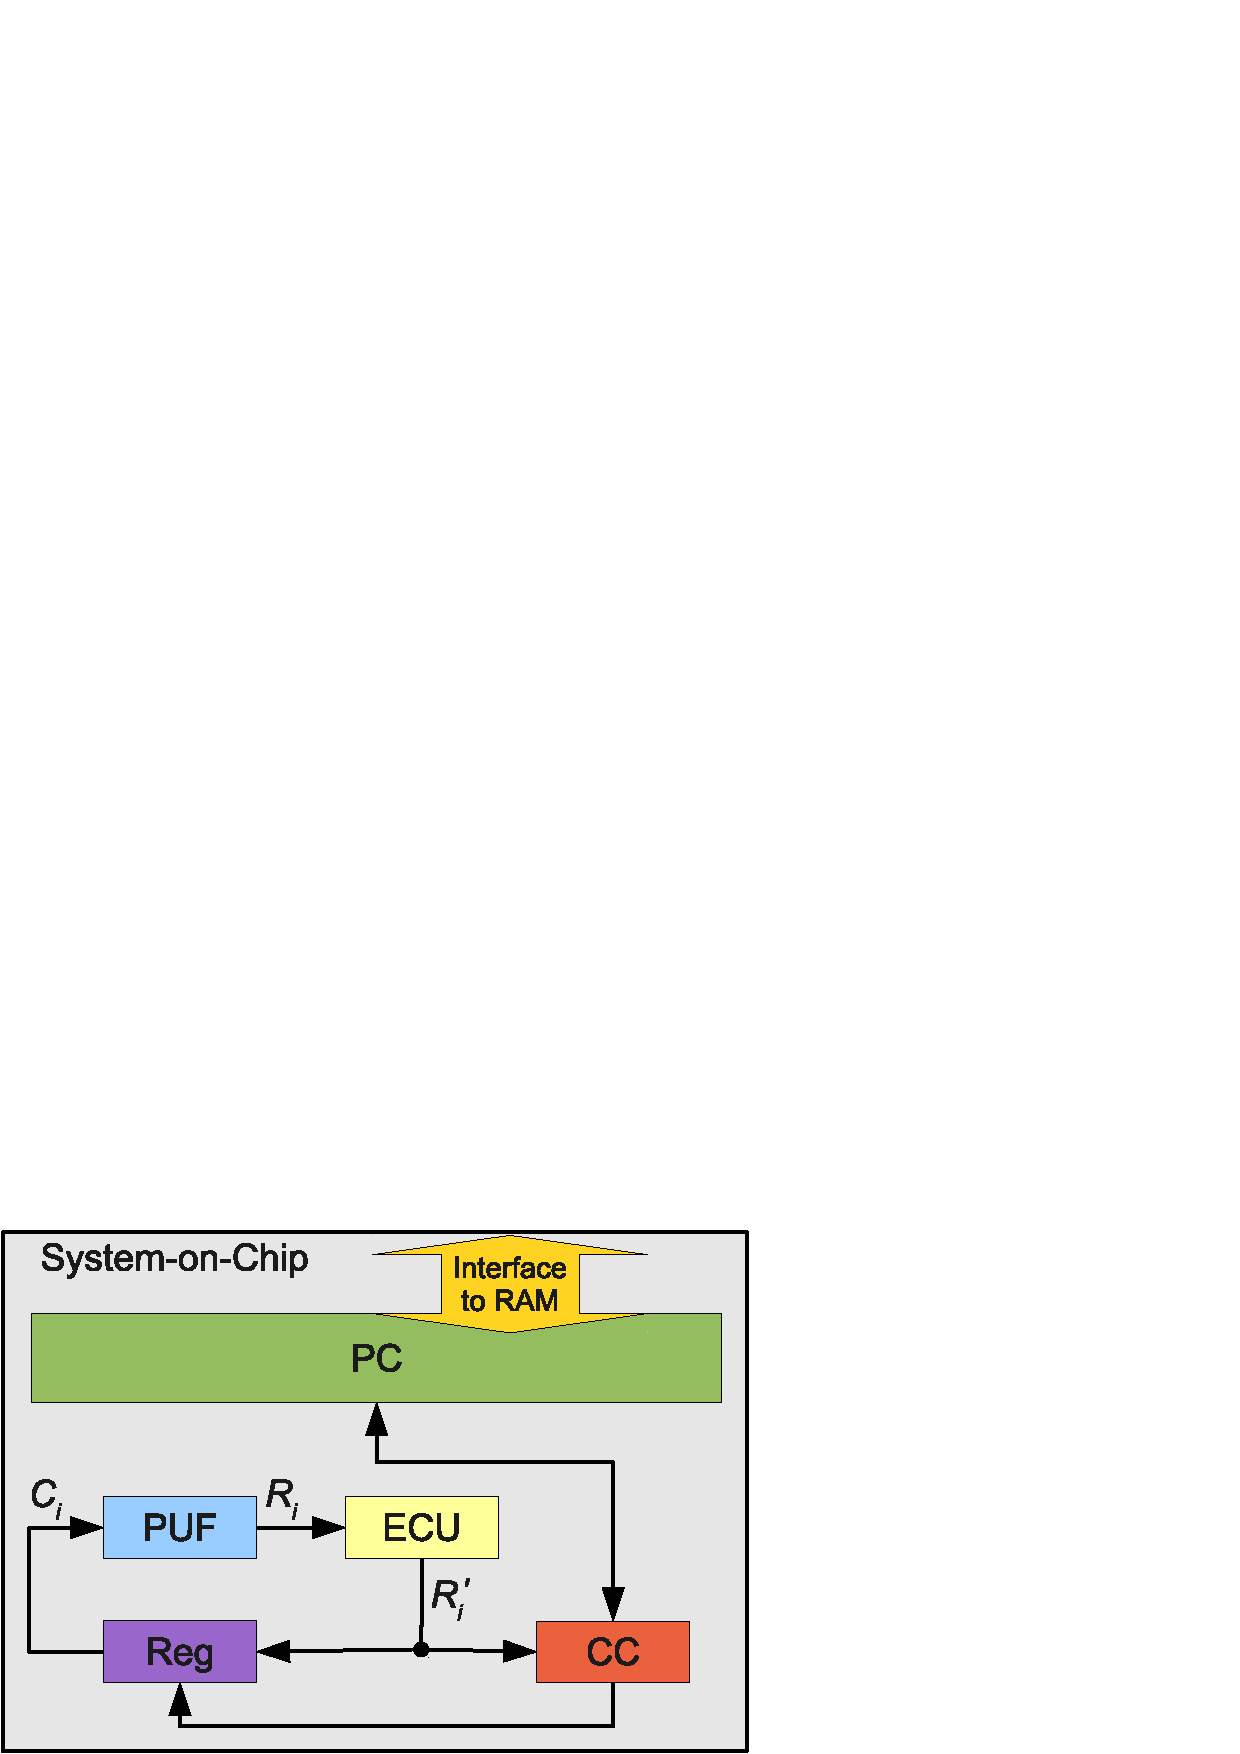
\includegraphics[width=500px]{images/rok_soc.pdf}
\label{fig:basicrok}
\caption{Block Level View of a Basic PUF ROK Device}
\end{figure}
\FloatBarrier

Upon a call to the encryption function, the PUF is executed with the contents of the register, error correction is stored,
and then the response overwrites the contents of the register. The response is also passed back to the cryptography
core where it can be used to generate an encryption key. This feedback loop ensures that once a key has been used
once, it cannot be used again, since it has been overwritten in the register.

When decryption is desired, the Init function must be used to re-seed the device so that the proper value is in the
register. Then, when Decrypt is called, the value in the register will be used as the challenge to the PUF, any errors
will be corrected by the error correction unit, and the result will overwrite the register and also be passed into the
CC. The response will then be used to derive the decryption key for the message.

\section{Security Considerations}

\section{Out of Order Execution}
One limitation of the basic PUF ROK design in~\ref{fig:basicrok} is that it does not allow out of order execution. That is,
if five messages are encrypted and then the third is requested to be decrypted, the PUF ROK must be re-seeded, the PUF
cycled twice, and then the third cycle can be used to actually perform the decryption. To decrypt the first message, the
PUF would again need to be re-seeded. 

Supposing this had to be done many times, this process would quickly become cumbersome. As such, it is desirable to
have a PUF ROK system that allows out of order execution. Figure~\ref{fig:rok} shows the block level design for a PUF
ROK that allows this out of order execution.

\begin{figure}[!ht]
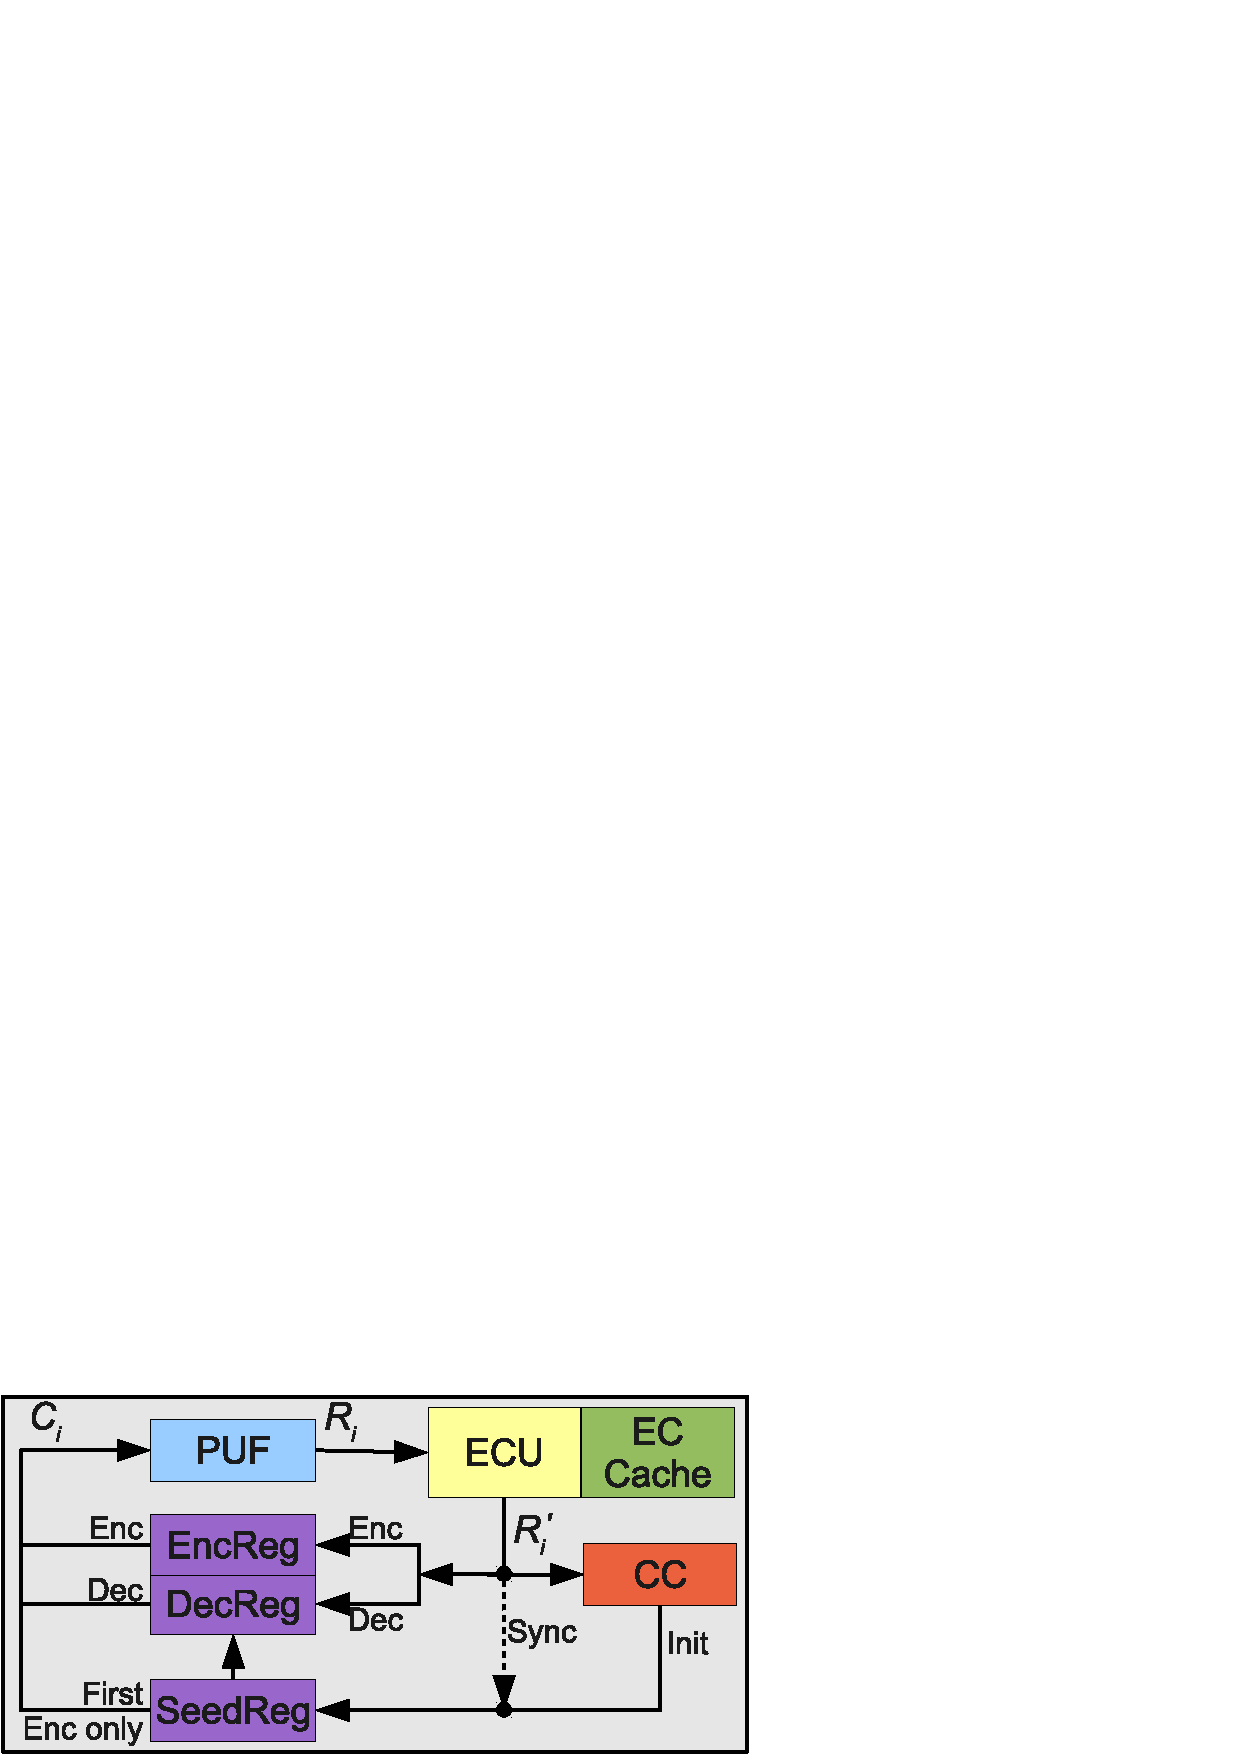
\includegraphics[width=500px]{images/rok_socreg.pdf}
\label{fig:rok}
\caption{Block Level View of a PUF ROK Allowing Out of Order Execution}
\end{figure}
\FloatBarrier

The modified PUF ROK is able to perform out of order executions by replacing the one original register with three
new registers, a seed register, an encryption register, and a decryption register. A cache is added to the error
correction unit as well. Note that all these new components are still internal to the PUF ROK design, so that no
buses are exposed externally.
The new design requires a new parameter, $N$. This parameter specifies the number of keys that will be stored in
the error correcting cache. The PUF ROK can then perform out of order execution on up to $N$ different keys.
The new design also introduces the Sync action, which is used to update the seed register and is further described
below.

Upon the initial seeding of the PUF ROK, the seed value is stored in the seed register. When the first encryption
is requested, the seed register is fed into the PUF. The response is then passed through error correction and stored
in both the error correcting cache as well as the encryption register. Note that the seed register is not updated here.
Upon request for another encryption, the contents of the encryption register will be used, rather than the seed register.

Upon a request for a decryption, if the requested key is still marked as valid in the error correcting cache,
the seed register is copied into the decryption register. The PUF is then cycled
and writes back to the decryption register enough times for the proper respone to be obtained. Note that the
error correcting unit is correcting any potential errors after each cycling of the PUF. At the conclusion of this, the
requested key is marked as used in the error correcting cache, meaning the PUF ROK will not use it again.

Because the error correcting cache has a finite amount of space, it will be necessary to clear the cache from time to
time. This is done using the Sync action. Sync is triggered when the first key in the cache has been marked as invalid.
(Note that this first key will be associated with the value currently in the seed register.) Since the values are invalid,
this means that they will never be used again, so the value in the seed register is obsolete and can be updated.
The error correction cache thus takes control of the feedback loop. It decides which key is the last used, and then cycles
the PUF, using the contents of the seed register that many times and writing the results back into the seed register.
For example, if there are 4 values stored in the cache and values 1 and 2 are invalid, the PUF will be cycled twice,
with the resulting response being written into the seed register.

\subsection{Security Implications}

\section{Implementation}
For a prototype implementation, the Saxo-L board from KNJN.com was used.~\cite{KNJN} It contains an Altera
Cyclone FPGA and an NXP LPC2132 ARM processor. The two chips are connected together by a Serial Peripheral
Interface (SPI). Additionally, a USB and a JTAG port are available, which makes for easy communication with the
various chips.

For the ease of development, we implemented only the PUF and the register on the FPGA and then implemented
the error correction unit, cryptography core, processor core, and other supporting computation on the ARM chip. 
When the PUF or register was needed, the ARM would issue a request over the SPI link to access the approprite component.
~\ref{fig:rokimpl} shows details of the implementation graphically.

\begin{figure}[!ht]
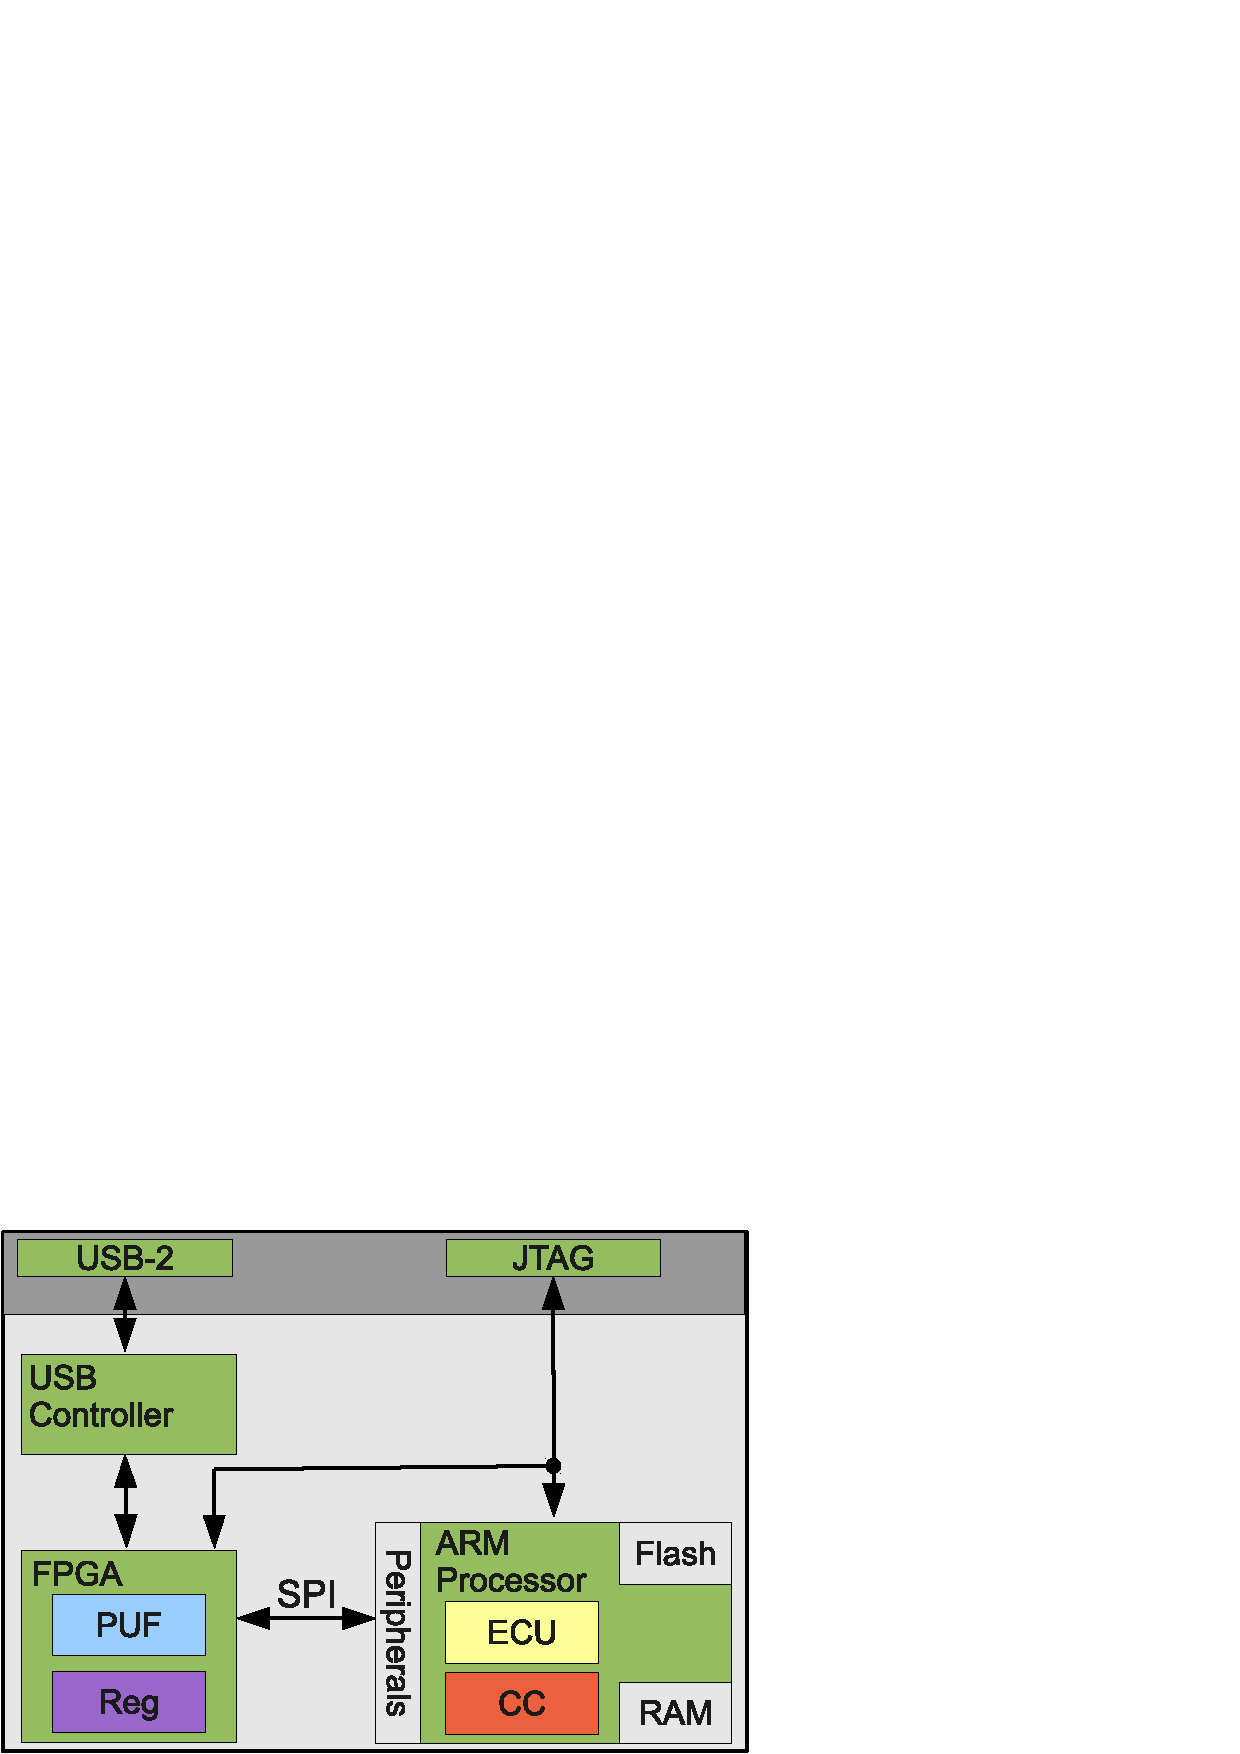
\includegraphics[width=500px]{images/rok.pdf}
\label{fig:rokimpl}
\caption{Implementation of a ROK device}
\end{figure}
\FloatBarrier

The Saxo-L board is 44 x 60 mm, which makes it very portable. A production quality device would likely be smaller.
This would allow the ROK to be implemented as a small dongle that could be plugged into a USB port potentially.

For the software portion of the project, the PolarSSL~\cite{polarssl} library was used, which is an SSL library
specifically optimized for small microprocessors, such as the LPC2132.

\subsection{Limitations}
There are some limitations to the implementation, since it is simply a prototype. The fact that the SPI bus is exposed
is a huge problem. As it currently exists, an attacker could simply attach logic probes to the bus and interecept or
modify any traffic between the FPGA and ARM chip. As such, he would be able to manipulate the values of the register
as well as what the error correction unit receives. Clearly, this is not a good thing.

This vulnerability could be mitigated by using some sort of tamper proofing, such as potting, but this is a relatively
expensive solution. Instead, the ideal solution would be to incorporate all the different components on one chip, as
shown in the original design. There are soft core ARM processors available which can be instantiated on an FPGA
already. It would be possible to simply move the entire ARM processor onto the same chip as the PUF and register.
Not only would this be more secure, but it would most likely be less expensive to manufacture a device with only
one chip, rather than two.

There are a variety of softcore microprocessors available, depending on the brand of FPGA selected, so there are
alternatives available to the ARM architecture.

\section{Results and Comparison}

\section{Future Work}
